\documentclass[twocolumn]{article}

% Packages
\usepackage{graphicx}
\usepackage{hyperref}
\usepackage{geometry}
\usepackage{amsmath}

% Additional package to allow for a subtitle
\usepackage[english]{babel}
\usepackage{titlesec}

% Page settings
\geometry{a4paper, margin=.75in}
\graphicspath{ {./images/} }

% Custom title and subtitle commands

\title{\vspace{-8ex}
    Dost \\ \vspace*{1ex}
  \large  CSE211 - Data Structures Term Project \\ \vspace*{1ex} Ahmet Hakan Candar \\ \vspace{1ex} 20220702022 \\ \vspace{-6ex}}

\date{}

% Document
\begin{document}

\maketitle


% Introduction
\section{Introduction}
This document serves as a comprehensive report of the Social Platforming App project. The project is a social networking platform written in C++ using the GTK4 and Adwaita frameworks. It is designed to provide users with a modern, user-friendly interface for connecting and interacting with others.

% Project Description
\section{Methodology}
The Social Platforming App project aims to create an interactive and intuitive platform for social networking. The app's main features include:
\begin{itemize}
    \item User authentication and account management.
    \item User profiles with customizable information.
    \item Social feed displaying posts from friends and followed accounts.
    \item Messaging functionality for direct communication between users.
    \item Search and discover features for finding new connections.
    \item Notifications and alerts for user interactions.
    \item Privacy and security settings for user data protection.
\end{itemize}

% Technologies Used
\section{Implementation}
The project is built using the following technologies:
\begin{itemize}
    \item **C++:** The main programming language used for the project.
    \item **GTK4:** The graphical user interface toolkit used for building the app's front-end.
    \item **Adwaita:** The design system used to create a modern, consistent UI for the app.
\end{itemize}

% Results
\section{Results}
\begin{tabular}{cc}
    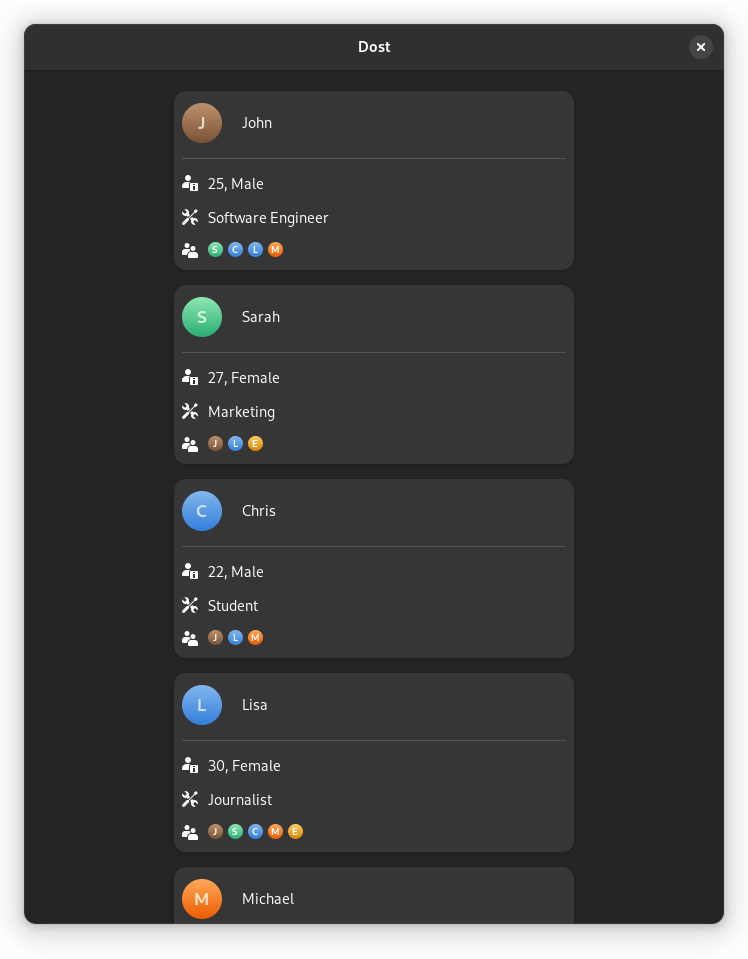
\includegraphics[width=.225\textwidth]{gui0} &
    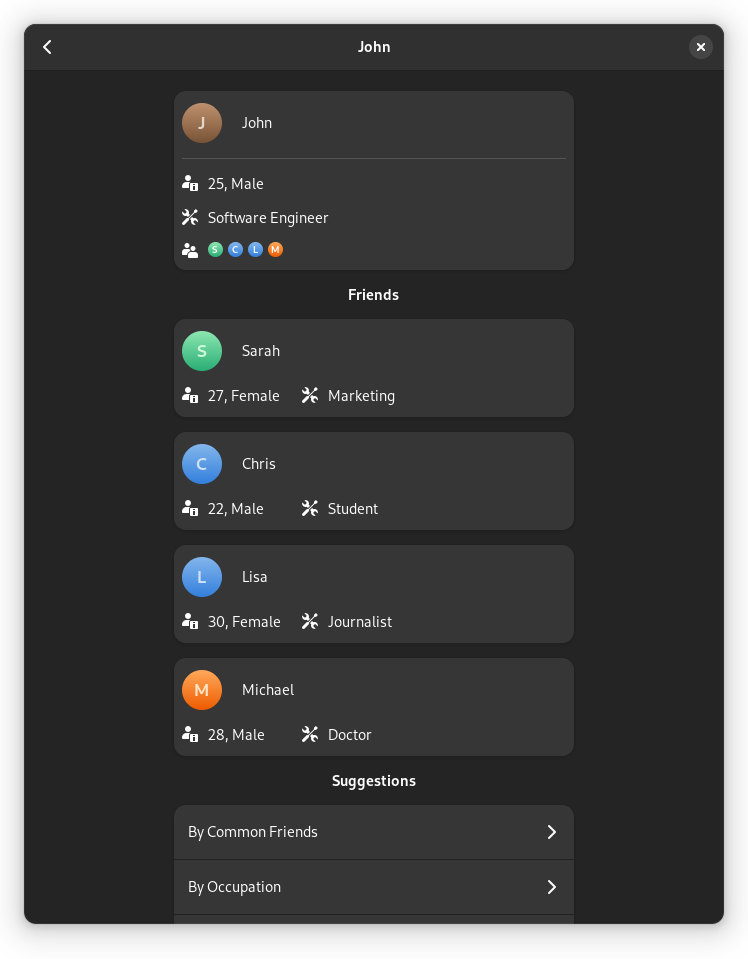
\includegraphics[width=.225\textwidth]{gui1}
     \\
     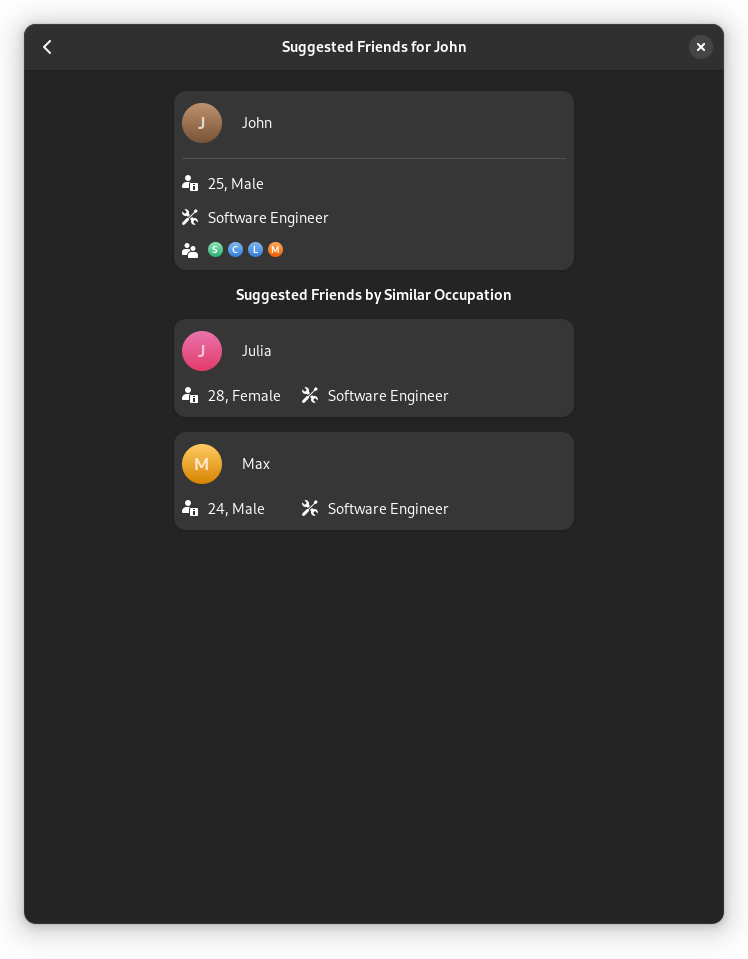
\includegraphics[width=.225\textwidth]{gui2} &
     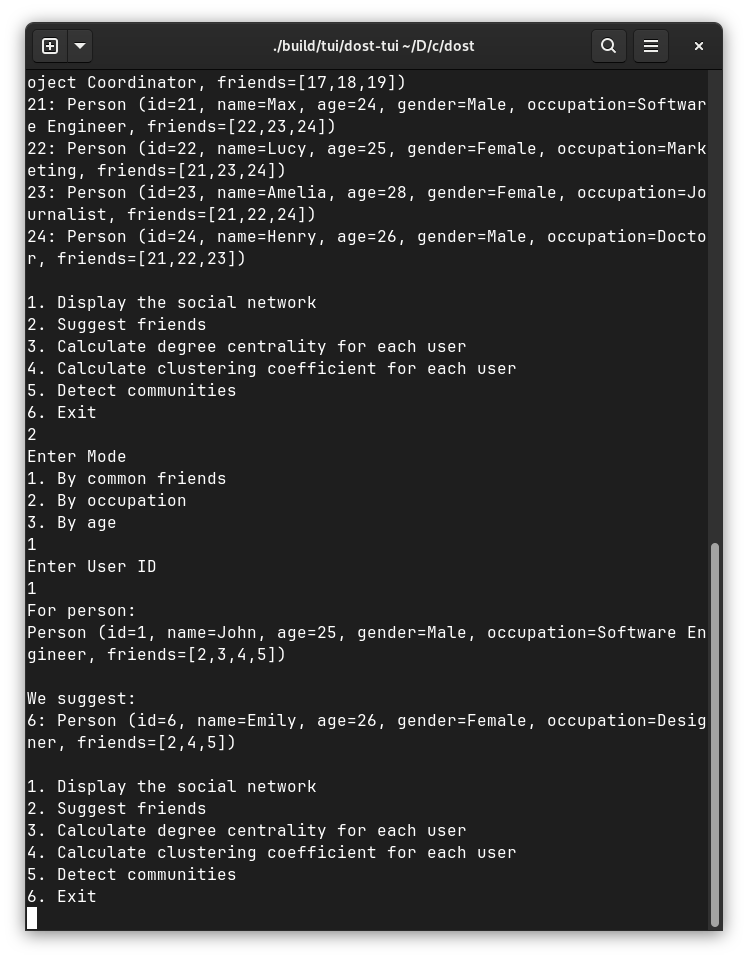
\includegraphics[width=.225\textwidth]{tui}
\end{tabular}
  
% Conclusion
\section{Conclusion}
Describe the challenges you faced during the development of the project and how you addressed them.

\end{document}
